\documentclass[../main.tex]{subfiles}

\graphicspath{{../images/}}

\begin{document}
\pagestyle{fancy}
\lhead{Lecture 2: 1/18}
\chead{Chapter 2}
\rhead{PHYS 472}

\section*{Chapter 2: Wave Diffraction and the Reciprocal Lattice}
\addcontentsline{toc}{section}{Chapter 2: Wave Diffraction and the Reciprocal Lattice}

% figure of bragg.png
\begin{figure}[ht]
    \centering
    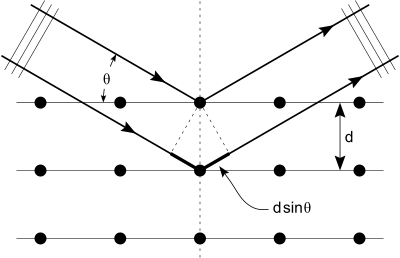
\includegraphics[width=0.4\linewidth]{bragg.png}
    \caption{Bragg's Law}
    \label{fig:2.1}
\end{figure}

\paragraph{Scattering and Bragg's Law}

When two beams of same phase meet, they constructively interfere. When they are out of phase, they
destructively interfere. The location of constructive interference, or path difference, is shown
by the bold lines in Figure \ref{fig:2.1}. The path difference is
\begin{align*}
    2d \sin \theta = n \lambda
\end{align*}
known as Bragg's Law which is only valid for $\lambda \leq 2d$. In reality each lattice plane will
reflect about $10^{-3} \sim 10^{-5}$ of the incident beam. Thus only about $10^3 \sim 10^5$ planes
contribute to the diffraction. The periodicity of the lattice leads to a periodic observable\dots

\emph{aside:} The electron wavefunction is not observable---$\psi$ is a complex number, but the
electron density, $\psi^* \psi$, is observable. Read about the quantized Hall effect (Queen):) and
Superconductivity (King).

\begin{align*}
    \psi(x + T) = \psi(x) e^{i\theta}
    n(x + T) = n(x)
\end{align*}

\paragraph{Fourier Transform} The discrete Fourier transfrom is useful for periodic functions.

\begin{align*}
    n(x) &= \sum_{P \geq 0} \qt[C_p \cos(\frac{2\pi}{a}x) + S_p \sin(\frac{2\pi}{a}x)] \\
    &= \sum_{p} n_p e^{i\frac{2\pi}{a}px}
\end{align*}
or in vector notation
\begin{align*}
    n(\vb{r}) = \sum_{\vb{G}} n_G e^{i\vb{G} \vdot \vb{r}}
\end{align*}
Since $n(x)$ is real, there is a symmetry of the complex conjugate
\begin{align*}
    n_p = n_{-p}^*
\end{align*}

\paragraph{Inverse Fourier Transform}
\begin{align*}
    n_p = \frac{1}{a} \int_0^a n(x) e^{-i\frac{2\pi}{a}px} \dd{x}
\end{align*}
and in vector notation
\begin{align*}
    n_G = \frac{1}{V} \int_{cell} n(\vb{r}) e^{-i\vb{G} \vdot \vb{r}} \dd{V}
\end{align*}

\paragraph{Reciprocal Space Vectors}

The basis vectors of the reciprocal lattice are
\begin{align*}
    \vb{b}_1 = 2\pi \frac{\vb{a}_2 \cross \vb{a}_3}{\vb{a}_1 \vdot (\vb{a}_2 \cross \vb{a}_3)};
    \quad \vb{b}_2 = 2\pi \frac{\vb{a}_3 \cross \vb{a}_1}{\vb{a}_1 \vdot (\vb{a}_2 \cross \vb{a}_3)};
    \quad \vb{b}_3 = 2\pi \frac{\vb{a}_1 \cross \vb{a}_2}{\vb{a}_1 \vdot (\vb{a}_2 \cross \vb{a}_3)}
\end{align*}
where the denominator is the volume of the unit cell (parallelpiped)
$\vb{a}_1 \vdot (\vb{a}_2 \cross \vb{a}_3) = V_c$.

Taking the dot product of a primitive vector with a reciprocal lattice vector gives
\begin{align*}
    \vb{a}_i \vdot \vb{b}_j = 2\pi \delta_{ij}
\end{align*}
where the Kronecker delta tells us that the dot product is either $2\pi$ or $0$. With this we can
write the $\vb{G}$ vector as a linear combination of the reciprocal lattice vectors
\begin{align*}
    \vb{G} = v_1\vb{b}_1 + v_2\vb{b}_2 + v_3\vb{b}_3
\end{align*}
we can also show that
\begin{align*}
    n(\vb{r} + \vb{T}) = n(\vb{r})
\end{align*}
which means that this is invariant under tranlsations.

\paragraph{Scattering amplitude}
\begin{align*}
    F = \int \dd{\vb{r}} n(\vb{r}) e^{i\vb{k} \vdot \vb{r}} e^{-i\vb{k}' \vdot \vb{r}}
\end{align*}
where $\abs{\vb{k}} = \abs{\vb{k}'}$. In vector notation
\begin{align*}
    F &= \int \dd{\vb{r}} \sum_{\vb{G}} n_G e^{i(\vb{G} - \vb{r}')} e^{-i\Delta\vb{k} \vdot \vb{r}} \\
    &= \sum_{\vb{G}} n_G \int \dd{\vb{r}} e^{i(\vb{G} - \Delta\vb{k}') \vdot \vb{r}} \\
\end{align*}
where $\Delta\vb{k} = -(\vb{k} - \vb{k}')$. When $\vb{G} = \Delta\vb{k}$ we can rewrite to
\begin{align*}
    \vb{k} + \Delta\vb{k} = \vb{k}'
\end{align*}
in absolute value
\begin{align*}
    \abs{\vb{k} + \Delta\vb{k}} = \abs{\vb{k}'} \rightarrow
    \abs{\vb{k} + \Delta\vb{k}} = \abs{\vb{k}} \rightarrow
    \abs{\vb{k} + \vb{G}} = \abs{\vb{k}}
\end{align*}
and
\begin{align*}
    (\vb{k} + \vb{G}) \vdot (\vb{k} + \vb{G}) = \vb{k} \vdot \vb{k} \rightarrow
    2\vb{k} \vdot \vb{G} + \vb{G}^2 = 0
\end{align*}
For the 1D crystal $G = 2\pi / a$. Since $\vb{k} \vdot \vb{G} = 2\pi/\lambda \vb{G} \sin\theta$
and $2\vb{k} \vdot \vb{G} = \vb{G}^2$
We get
\begin{align*}
    2 \vdot \frac{2\pi}{\lambda} G \sin\theta &= \vb{G}^2 \\
    \rightarrow \frac{4\pi}{\lambda} \sin\theta &= G 
\end{align*}
since $G = 2\pi / a$ we get Bragg's Law
\begin{align*}
    2d \sin\theta = n\lambda
\end{align*}
For the SC the reciprocal lattice is SC, but for BCC, the reciprocal lattice is different\dots

\newpage
\lhead{Lecture 3: 1/23}

\section*{Chapter 2: cont'd}

\paragraph{Wigner-Seitz primitive cell:} How to create the most symmetric primitive cell.

% figure of pcell.png
\begin{figure}[ht]
    \centering
    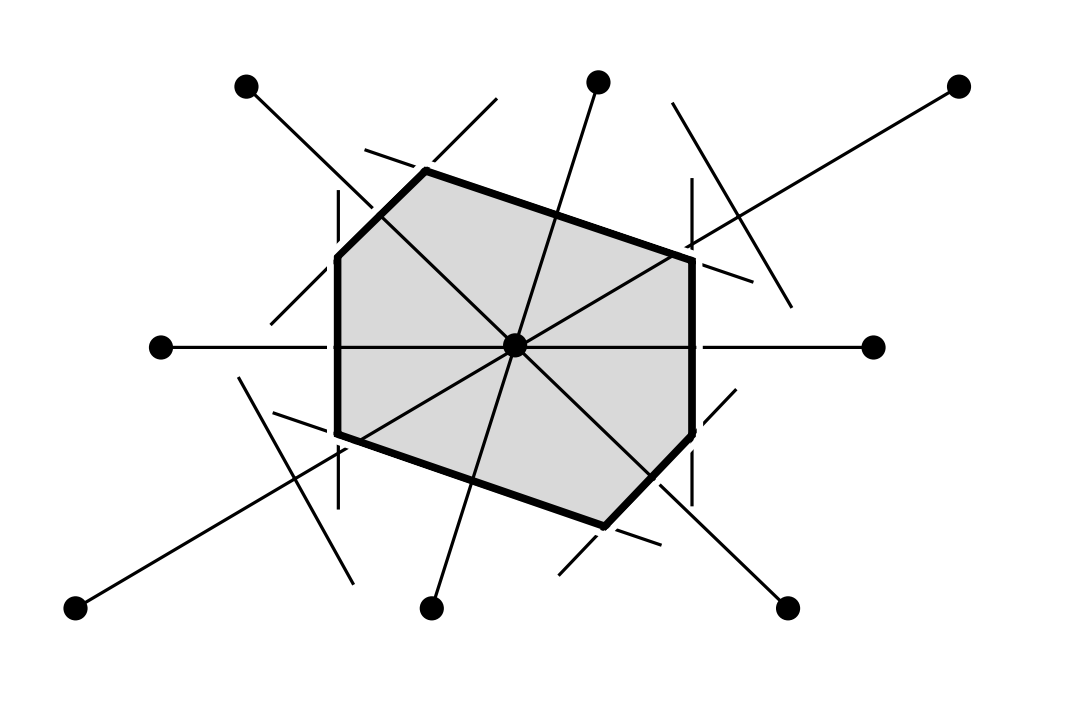
\includegraphics[width=0.4\linewidth]{pcell.png}
    \caption{Wigner-Seitz Primitive Cell}
    \label{fig:3.1}
\end{figure}
Steps: Connect a given lattice point to all nearby lattice points. Bisect all lines. The area 
enclosed by the bisectors is the Wigner-Seitz primitive cell as shown in Figure \ref{fig:3.1}.

\paragraph{Reciprocal Lattice of SC} The lattice vectors (primitive translation vectors) are
\begin{align*}
    \vb{a}_1 = a\vu{x}, \quad \vb{a}_2 = a\vu{y}, \quad \vb{a}_3 = a\vu{z}
\end{align*}
the reciprocal lattice vectors using the formula from last lecture are
\begin{align*}
    \vb{b}_1 = 2\pi \frac{\vb{a}_2 \cross \vb{a}_3}{V_c} = \frac{2\pi}{a}\vu{x}, \quad
    \vb{b}_2 = \frac{2\pi}{a}\vu{y}, \quad \vb{b}_3 = \frac{2\pi}{a}\vu{z}
\end{align*}

\paragraph{Reciprocal Lattice of BCC} The lattice vectors are
\begin{align*}
    \vb{a}_1 = \frac{a}{2}(-\vu{x} + \vu{y} + \vu{z}), \quad
    \vb{a}_2 = \frac{a}{2}(\vu{x} - \vu{y} + \vu{z}), \quad
    \vb{a}_3 = \frac{a}{2}(\vu{x} + \vu{y} - \vu{z})
\end{align*}
and the reciprocal lattice vectors are
\begin{align*}
    \vb{b}_1 = \frac{2\pi}{a}(\vu{y} + \vu{z}), \quad
    \vb{b}_2 = \frac{2\pi}{a}(\vu{z} + \vu{x}), \quad
    \vb{b}_3 = \frac{2\pi}{a}(\vu{x} + \vu{y})
\end{align*}

\paragraph{Reciprocal Lattice of FCC} The lattice vectors are
\begin{align*}
    \vb{a}_1 = \frac{a}{2}(\vu{y} + \vu{z}), \quad
    \vb{a}_2 = \frac{a}{2}(\vu{x} + \vu{z}), \quad
    \vb{a}_3 = \frac{a}{2}(\vu{x} + \vu{y})
\end{align*}
which is the same as the reciprocal space of BCC. Thus, the reciprocal lattice of FCC is BCC!

\paragraph{Brillouin Zone} The first Brillouin zone is the Wigner-Seitz primitive cell of the
reciprocal lattice.
\end{document}